\pagestyle{kalinka}
\label{kalinka}

\begin{textblock*}{5.625in}(0pt,0pt)%
\vspace*{-1.45cm}
\hspace*{-1.2cm}\includegraphics*[width=112mm]{./imgs/KALINKA.png}
\end{textblock*}

\pagebreak

\hspace{.5cm}

\begin{center}
\hspace*{-.5cm}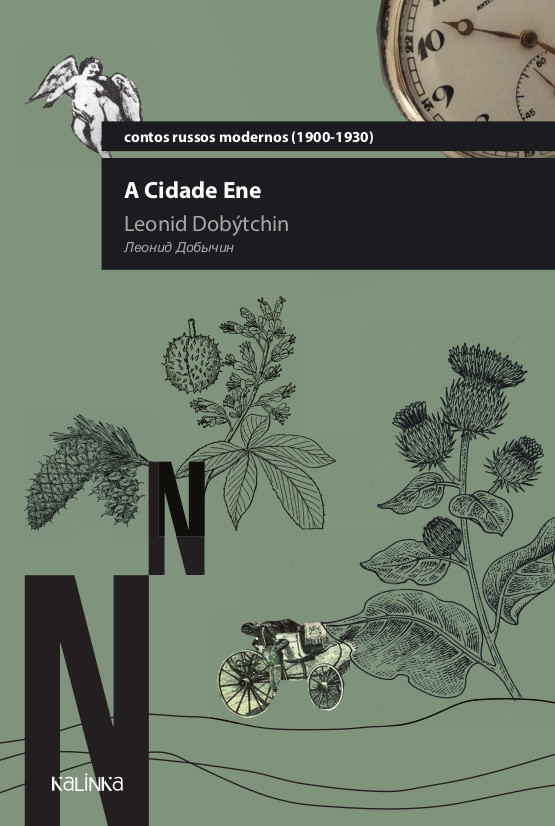
\includegraphics[width=45mm]{./imgs/cidaden.jpeg}
\end{center}

\hspace*{-2cm}\_\_\_\_\_\_\_\_\_\_\_\_\_\_\_\_\_\_\_\_\_\_\_\_\_\_\_\_\_\_\_\_\_\_\_\_\_\_\_\_\_\_\_\_\_\_\_\_\_\_\_\_\_\_\_\_\_\_\_\_\_\_\_\_\_\_\_\_\_\_\_\_\_\_

\medskip

\noindent{}De traços autobiográficos, {\slsc{A Cidade Ene}} traz uma narrativa do ponto de vista de uma criança do começo do séc. \scalebox{.8}{XX}. Desvelam"-se reminiscências de uma Rússia pré"-revolucionária, e sua burguesia decadente e provinciana. Leonid Dobýtchin (1894-1936), genial modernista russo, criou uma obra com detalhes que se imprimem no texto como manchas de uma pintura pontilhista, “criando um panorama complexo e harmônico”, como escreve Richard Borden.

\vfill

\hspace*{-.4cm}\begin{minipage}[c]{0.45\linewidth}
\small{
{\Formular{\textbf{
\hspace*{-.1cm}Título: A cidade Ene\\
Autor: Leonid Dobýtchin\\ 
Editora: Kalinka\\
Páginas: 180\\
Formato: 14x21cm\\
Preço: R\$ 46,90\\
ISBN: 978-85-6109-620-0
}}}}
\end{minipage}

\pagebreak





%\hspace{.5cm}
%
%\begin{center}
%\hspace*{-1cm}\raisebox{5.5cm}{\rotatebox[origin=t]{90}{\Formular{\textbf{Lançamento}}}}
%\hspace{1cm}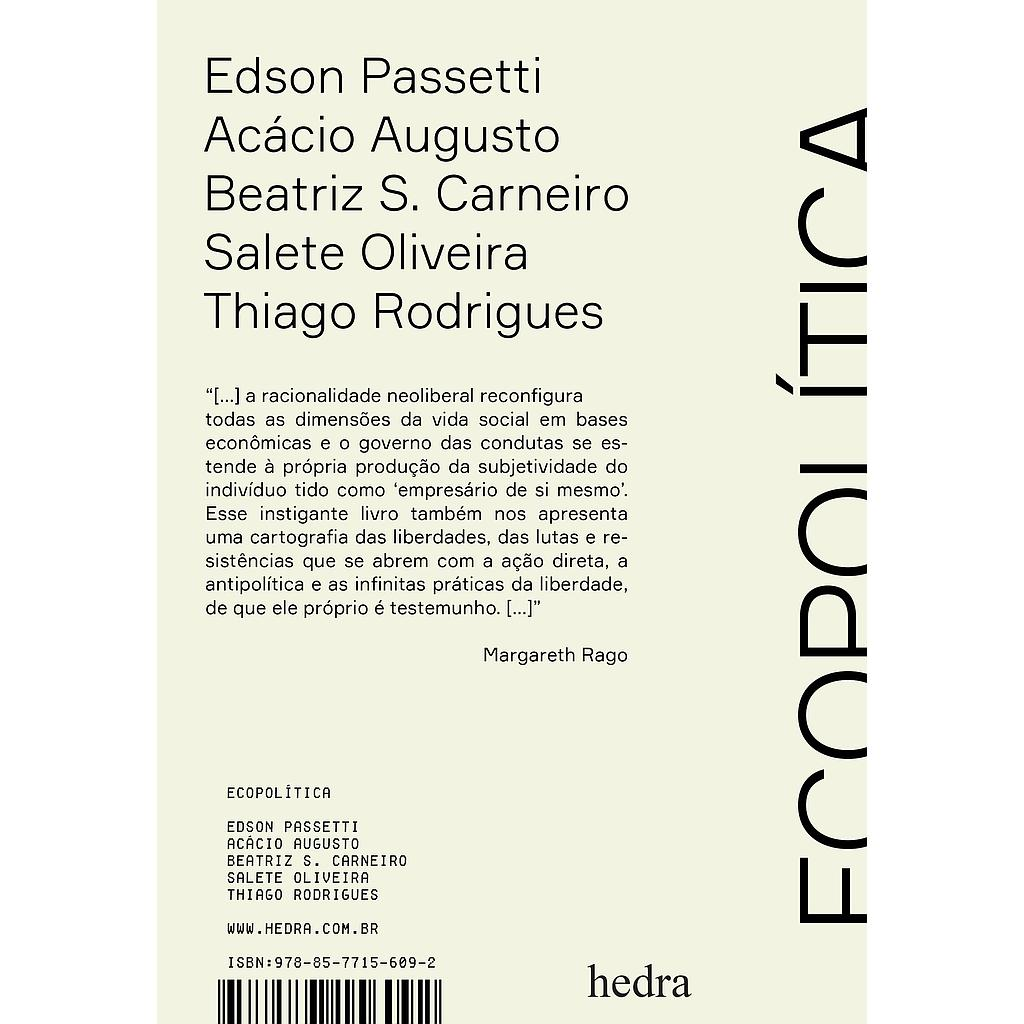
\includegraphics[width=70mm]{eco.jpeg}
%\end{center}
%
%\hspace*{-2cm}\_\_\_\_\_\_\_\_\_\_\_\_\_\_\_\_\_\_\_\_\_\_\_\_\_\_\_\_\_\_\_\_\_\_\_\_\_\_\%_\_\_\_\_\_\_\_\_\_\_\_\_\_\_\_\_\_\_\_\_\_\_\_\_\_\_\_\_\_\_\_\_\_\_\_
%
%\medskip
%
%\noindent{}Lorem ipsum dolor sit amet, consectetur adipiscing elit.
%Donec sodales tortor a purus accumsan, ut ultricies purus
%maximus. Aliquam bibendum consequat mi, sed commo-
%do velit pellentesque id. Vivamus ultricies ligula in semper
%sagittis. Donec mollis odio in lectus tristique, sed convallis
%est interdum. Cras eget sem condimentum, pretium purus
%eu, auctor.
%
%\hspace{.5cm}
%
%\hspace*{-.4cm}\begin{minipage}[c]{0.45\linewidth}
%\small{
%{\Formular{\textbf{
%\hspace*{-.1cm}Título: Ecopolítica\\
%Autor: Edson Passetti\\ 
%Editora: Hedra\\
%Páginas: 476\\
%Formato: 23x16cm\\
%Preço: R\$ 79,90\\
%}}}}
%\end{minipage}
%\begin{minipage}[c]{0.50\linewidth}
%\small{Lorem ipsum dolor sit amet, consectetur adipiscing elit. Donec sodales tortor a purus accumsan, ut ultricies. Lorem ipsum dolor sit amet, %consectetur adipiscing elit. Lorem ipsum dolor sit amet. Lorem ipsum dolor sit amet.} 
%\end{minipage}
%
%\pagebreak
%
%\hspace{.5cm}
%
%\begin{center}
%\hspace*{-.5cm}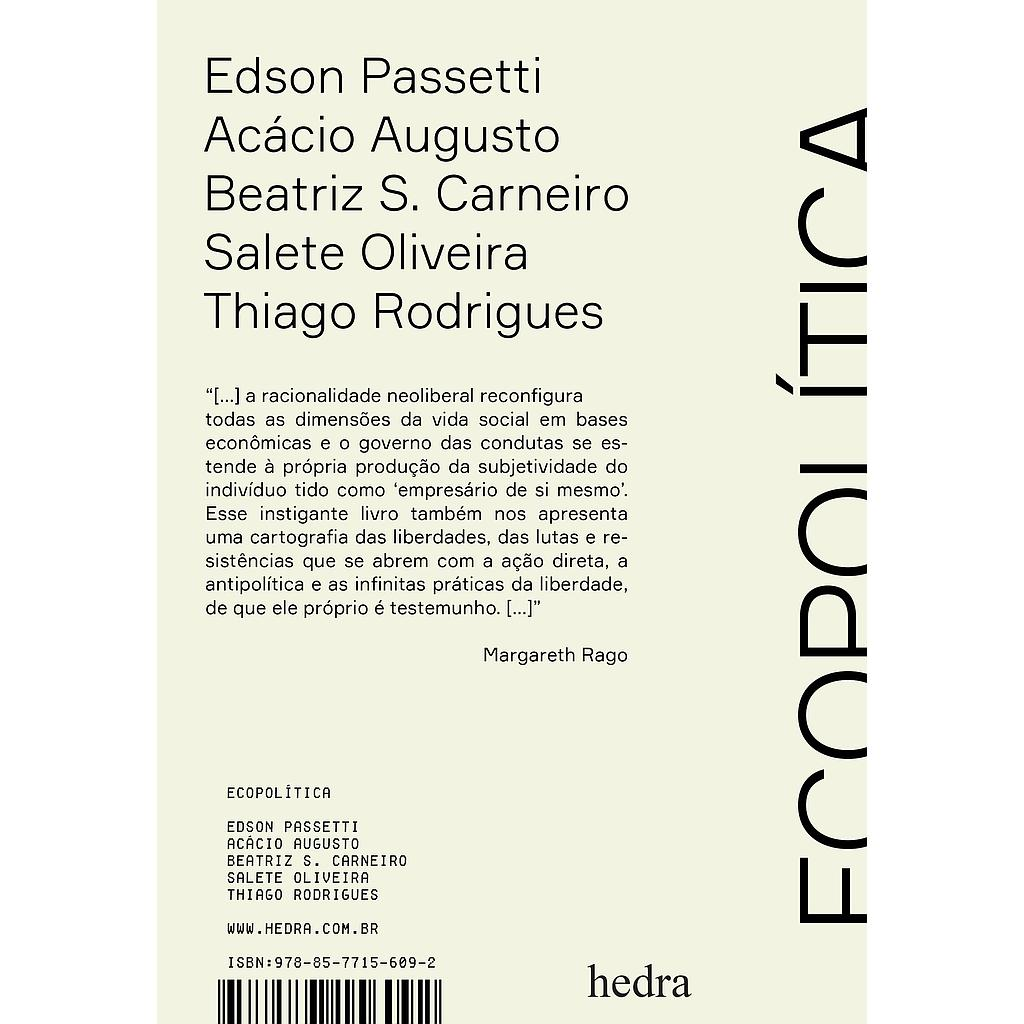
\includegraphics[width=70mm]{eco.jpeg}
%%\hspace*{6cm}\raisebox{2cm}{\rotatebox[origin=t]{90}{\Formular{\textbf{Lançamento}}}}
%\end{center}
%
%\hspace*{-2cm}\_\_\_\_\_\_\_\_\_\_\_\_\_\_\_\_\_\_\_\_\_\_\_\_\_\_\_\_\_\_\_\_\_\_\_\_\_\_\%_\_\_\_\_\_\_\_\_\_\_\_\_\_\_\_\_\_\_\_\_\_\_\_\_\_\_\_\_\_\_\_\_\_\_\_
%
%\medskip
%
%\noindent{}Lorem ipsum dolor sit amet, consectetur adipiscing elit.
%Donec sodales tortor a purus accumsan, ut ultricies purus
%maximus. Aliquam bibendum consequat mi, sed commo-
%do velit pellentesque id. Vivamus ultricies ligula in semper
%sagittis. Donec mollis odio in lectus tristique, sed convallis
%est interdum. Cras eget sem condimentum, pretium purus
%eu, auctor.
%
%\hspace{.5cm}
%
%\hspace*{-.4cm}\begin{minipage}[c]{0.45\linewidth}
%\small{
%{\Formular{\textbf{
%\hspace*{-.1cm}Título: Ecopolítica\\
%Autor: Edson Passetti\\ 
%Editora: Hedra\\
%Páginas: 476\\
%Formato: 23x16cm\\
%Preço: R\$ 79,90\\
%}}}}
%\end{minipage}
%\begin{minipage}[c]{0.50\linewidth}
%\small{Lorem ipsum dolor sit amet, consectetur adipiscing elit. Donec sodales tortor a purus accumsan, ut ultricies. Lorem ipsum dolor sit amet, %consectetur adipiscing elit. Lorem ipsum dolor sit amet. Lorem ipsum dolor sit amet.} 
%\end{minipage}
%
%\pagebreak